\chapter{Instrument Suite}

* Total mass and power requirement

* What do we want to measure and why? Explain why some instruments were picked and some were discarded (we can use the notes from when we did that in class)

\section{Up-concentration}

* Petri Dish can be used for cultivation

\section{Water flow for the instruments} % Figure out a better title?

* Water convection is not enough. We need a pump (peristaltic pump).

\section{Sample handling}

* We need a design, I (Kristian) talked with some other about this, but we need to coordinate with the rest of the groups
   (SMS http://www.esmats.eu/amspapers/pastpapers/pdfs/2008/mumm.pdf)

* Sample rate

* What is under pressure and what is not?

* Order of the instruments

\subsection{Robot Arm} % Rasmus


\section{CTD/ADCP} % Sridhar

* Includes temperature probe

    * We will properly need more around the body of the penetrator

\section{Light sensor}

\autsection{Gas detector}{Agge Winther}

This chapter concentrates on why gas detection is important when searching for life, and how an instrument is designed for use in the penetrator to detect different gasses.

First a look into what gasses to be expected on Europa, next a look into gas detection under normal circumstances, and lastly a design of a gas detector for specific use in the ocean of Europa.

\subsection{Theory}

The main objective for this mission is to search for life. As explained in earlier chapters this could be found in many shapes and sizes. From bacteria to small living organisms, or perhaps alien life forms, unknown to science. If Europa is a life harbouring planet, and the ocean under the ice contains some sort of life. Then it would be an idea to also investigate extinct life.

Assuming the type of life can be compared to that of earth, we should be able to detect bi-products from living organisms. This chapter focuses on gasses, produced by living organisms, decomposed organic material or nutrients to support life.

As know from life and living organisms on earth, most life depend on the sun to create some sort of photosynthesis. Under the ice of Europa little to no light is expected to be found due to the thickness of the ice sheet above. Therefore traditional life, driven by the sun, is not to be found in the water of Europa, but for life harbouring conditions, some energy must be available.

Look back at earth, only a few places exist where life thrives, without light. One of them is around the black smokers on the ocean floor. The reason for mentioning this example is that Europa studies\cite{schmidtocean} show that a source of energy could be similar to the black smokers on earth. Life is found in great abundance around the smokers. First it was thought the organisms lived on marine snow, but the amount of life compared to the little amount of marine snow, would not be able to sustain the large amount of organisms found. Now it is know that the organisms thrive on the bacteria living around the smokers. This is called chemosynthetic bacteria, and instead of using photosynthesis the bacteria uses the nutrients and hydrothermal fluids from the smokers. The bacteria uses sulfur, methane and heat the create the energy need for life, this then feeds other life like clams and tubeworms, and usually a small ecosystem is found around black smokers, even if there is now sunlight. Some of the organisms around the smokers do depend on oxygen but anaerobic organisms are also found\cite{PMEL}.

This is good indication for life and even if the smokers are long gone, decomposition of the bacteria and ecosystems around the smokers could be seen in the levels of sulfur, methane, ethane, $CO_2$ and other hydrocarbons found in the water. Therefore sensors which can detect hydrocarbons would be ideal to bring with the penetrator down to the ocean, and look for these gasses.

\subsubsection{Searching for hydrocarbons}

Hydrocarbons are organic compounds made from carbon and hydrogen. Overall hydrocarbons can be dived in the 4 groups:
\begin{itemize}
  \item Saturated hydrocarbons (alkanes)
  \item Unsaturated hydrocarbons (alkenes)
  \item Cycloalkanes
  \item Aromatic Saturated hydrocarbons
\end{itemize}
Where methane and ethane is alkane's due to their single bond. On Earth most hydrocarbons come from decomposed organic matter, and it is this connection that will help conclude the kind of life on Europa.

Taking into account the smokers, organic material and simple life forms, simple hydrocarbons and other gasses would be found dissolve in the water or as gas bubbles. From this point on the focus shift towards detecting these gasses, which include: $SO_2$, H2S, $CH_4$, $NH_3$, $CO_2$, C2H6. The sensor need to be design must be able to detect as many as possible and if feasible, even bigger alkenes, alkanes and aromatic compounds.

\subsubsection{Detecting hydrocarbons at low pressure}

Detecting hydrocarbons can be done in many ways, first a look into how detection of gasses is done on Earth. This will give an idea on how today's methods could be modified and implemented in the instrument suite on the penetrator.

Most gas detectors are used to detect gasses harmful to humans, and leaks in pipelines. Most detectors are used to detect gasses in industry for safety reasons, helping to detect toxic, flammables or oxygen depletion, dangerous to workers or work safety. The most common ways to detect gas are:
\begin{itemize}
  \item Electrochemical
  \item Infrared
  \item Semiconductor sensor
  \item Ultrasonic
  \item Holographic
\end{itemize}
Electrochemical gas detectors diffuses the gas through a membrane, into an electrode, where it is oxidized. The reaction between the electrode and the gas generates an electric current which is linear to the gas concentration and by changing the membrane it is possible to custom design a detector for a specific gas. This type of sensor is very simple, stable and robust, but it is not perfect, it suffers from cross sensitivity and if it gets in contact with corrosive compounds, its life of operation is shortened\cite{intlsensor}.

Infrared gas detecting uses a whole other method to determining the gas in question. Here infrared light is passed through a known volume of gas, and the absorption of the different wavelength in the infrared spectrum is then analyzed. Different gasses have different absorption spectrums, like a fingerprint, and thereby the gas can be determined. This technique is more complex, but a lot more flexible compared to the electrochemical sensor, since it is able to detect different gasses with the same detector\cite{ndir}.

Semiconductor sensors detect gas by a chemical reaction with the semiconductor material, most used is tin-oxide, as gas comes in contact with the tin-oxide the resistance through the material drops. This type of sensor is commonly used for detection of methane, carbon monoxide, hydrogen, oxygen and alcohol-vapor.

Ultrasonic gas detectors are mostly used for detecting leaks, and cannot determine gas concentration. It works by listing for changes in the background noise around ultrasonic frequencies, since high pressure gas-leaks emit ultrasonic sounds, which can be detected. It is therefore no good for the type of detection wanted for this mission.

Lastly there are holographic gas sensors; they work under much the same principle as for the infrared detectors. Here the change in the reflected wavelength from the hologram can be used to determine the composition of the gas in front of the hologram. To work, they do require white light or lasers, which makes them more complex then the infrared sensors.

All of these methods mention above can be used on a gas, but a gas is just a state of the specific compound in question. On earth the gasses mentioned previously ($SO_2$, H2S, $CH_4$, $NH_3$, $CO_2$, C2H6) are naturally occurring as gas at sea level, (1 atm, 20 C), but this is not the case at the crushing pressure under the ice.

\subsubsection{Gas detection at Europas ice-sea surface}

The exact composition of Europas internal geology is still unknown. Qualified guess can be made dependant on pictures and its orbit. From this, it is estimated that the ice could be proximately 10km thick, all this ice generate an enormous pressure, estimated to be between 100-200bars at the ice-water barrier. Therefore what on Earth is a gas, would be a liquid or supercritical where the penetrator is sitting analyzing samples. To get a better insight into what happens to a compound mixed with water under this pressure a small study is done below.

At the ice-water barrier the temperature is around 273.15 Kelvin, below this the water starts to freeze and above it melts at a pressure of 100 bar\cite{PhaseH20}. At 200bar the temperature will be a 3 to 5 degrees Kelvin lower due to the pressure, but in general the freezing temperature is constant\footnote{This is for pure $H_2 O$}.

Overall a substance can have 3 states, gas, liquid or solid, it can also become super critical where it is in-between all 3 states. The way to characterize the states of a substance is through its phase diagram. An example of this is $CO_2$, which have the following phase diagram.

\begin{figure}[htb]
  \centering
  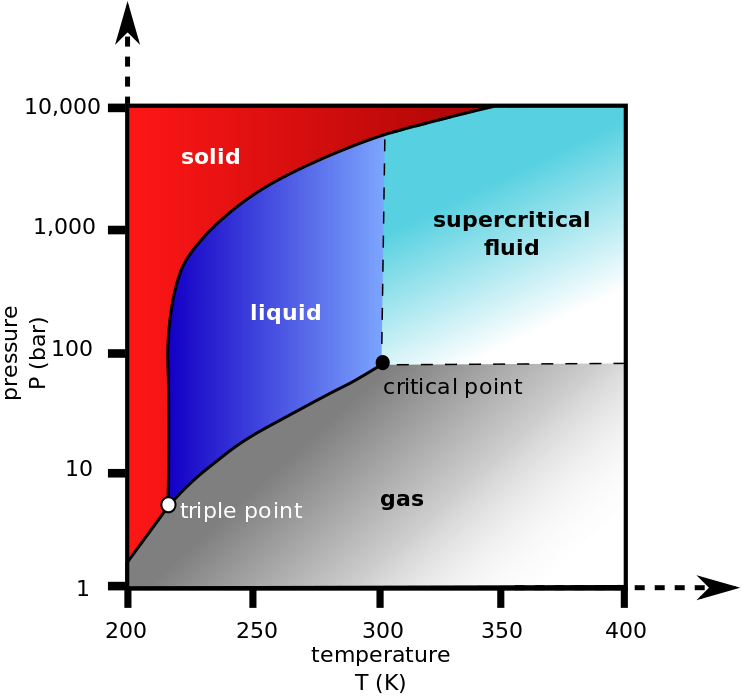
\includegraphics[scale=0.4]{figures/GasDetectionAgge/CO2PhaseDiagram}
  \caption{Phase diagram of $CO_2$, here the different phases are clearly seen, and how they depend on pressure and temperature\cite{PhaseCO2}}
  \label{fig:PhaseDiagramCO2}
\end{figure}

In the phase diagram of $CO_2$ (\ref{fig:PhaseDiagramCO2})it can be seen how the phases depend on pressure and temperature. If there is $CO_2$ present in the water at Europa, it would not be as a gas, because at 100 bar and 273.15 Kelvin $CO_2$ is liquid.

If $CO_2$ is present in the water, it is most likely to be mixed in the water, since water is a very good solvent for ionic and organic compounds, which makes most substances soluble in water; this is also the case for the gasses in question here. The solubility of substance in the water depends on the pressure above the solution. This follows Henry's law which states that the "solubility if a gas in liquid is directly proportional to the pressure above the surface of the solution\cite{SolubilityOfGases}".

This can be demonstrated with a bottle of soda. When the bottle is opened the pressure is released and CO2 starts to bubble up because the water cannot contain the same amount of $CO_2$ in the soda, under 1atm pressure.
As the phase diagram, a graph of the solubility of a substance can be made; here it is the solubility of $CO_2$ in water, but at atmospheric pressure:

\begin{figure}[htb]
  \centering
  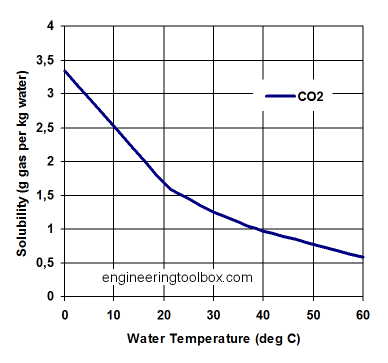
\includegraphics[scale=0.4]{figures/GasDetectionAgge/CO2Solubility}
  \caption{The solubility of $CO_2$ gas in water, at atmospheric pressure\cite{SolubilityOfGasesInWater}}
  \label{fig:SolubilityofCO2}
\end{figure}

From \ref{fig:SolubilityofCO2} it is seen that approximately 3.4 grams of $CO_2$ gas can solute in water at 273.15 Kelvin at a pressure of 1 atm. Combining this with Henry's law, the amount increases proportionally with the pressure, so the amount of $CO_2$ the water is able to solute is grater at 100 bar. Even when the $CO_2$ is liquid the solubility can be approximated as a gas/liquid solution\cite{SolubilityExplained}.

The conclusion on this is, it is not possible to use "normal" gas detecting methods, as discussed above. Other methods are needed to be able to detect what substances are present in the water. Some of the substances like $CO_2$ and $SO_2$ will be a liquid mixed with water, others might be a gas or super critical. The way of detecting the substances in the water needs to be done on another way.

\subsection{Implementation}

From the theory section it was discussed how to detect gasses, and what problems, and complications this have at high pressure, between the water and ice at Europa. The main problem in gas detection at Europa, concerned the fact that most of the gasses are liquid and not a gas. Therefore an instrument is design to take advantage of this high pressure condition. First the substances of interest are indexed according to their phase, solubility and at what pressure they change phase from liquid to gas (at constant temperature of 273.15 K) under the ice. Here the assumption is 100 bar and 273.15 degrees Kelvin.

\begin{table}
  \resizebox{\textwidth}{!}{%
  \begin{tabular}{|c | c | c | c|}
    \hline
     Substance: & Solubility: (g/kg water) & State: & Phase change pressure\cite{GasEncyclopedia} [Bar] \\ [0.5ex]
    \hline
    $SO_2$ (Sulfur dioxide) & 225 & Liquid & 1.5\\
    \hline
    $CO_2$ (carbon dioxide) & 3.4 & Liquid & 35\\
    \hline
    $NH_3$ (Ammonia) & 900 & Liquid & 4\\
    \hline
    $H_2 S$ (Hydrogen sulfide) & 7 & Liquid & 6\\
    \hline
    $C2H6$ (Ethane) & 0.13 & Liquid & 25\\
    \hline
    $CH_4$ (Methane) & 0.04 & Gas/Super & NA\\
    \hline
  \end{tabular}}
\end{table}

As mention in the Theory section, these substances are of great interest to detect possible life/extinct life in the water, for now on the focus will be on these 6 compounds for the further development of an instrument for the penetrator.

From the table above it is noted that all of the compounds are soluble in water, and most of them as a liquid at 100 bar and above. The notable characteristic is the phase change pressure, where the liquid changes phase to a gas. The important thing here is different pressures where the phase change happens, as for the IR-gas detector, this is a fingerprint tied to the compound. The odd one out is methane, it is still in a gas or supercritical state; it could therefore be detected with standard methods already known.  This will be investigated later.

The idea is to use an expansion chamber to boil of the gasses by lowering the pressure slowly. In constant temperature conditions a slow expansion of the gas, will give a characteristic pressure graph, with flat spots as the compound boils off and changes it phase. The principle can be seen in \ref{fig:PVdiagram} below.

\begin{figure}[htb]
  \centering
  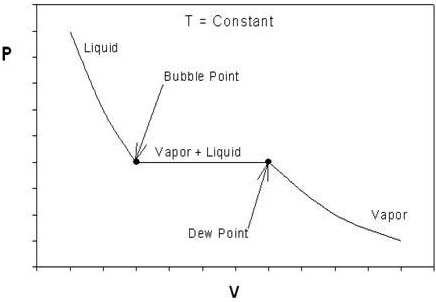
\includegraphics[scale=1]{figures/GasDetectionAgge/PVdiagram}
  \caption{PV-diagram with constant temperature. As the volume expands, the pressure drops, and the liquid changes state into gas}
  \label{fig:PVdiagram}
\end{figure}

In the PV-diagram, going from left to right, the liquid follows an isotherm as the pressure drops, when it reaches it phase change, and the liquid boils of into a gas. As this happens the pressure remains constant. With the help of a pressure sensor this can be detected, and the gas identified.

To create this phase change the pressure of the liquid under test needs to be dropped. If an expansion chamber is used then the Europa's liquid water will enter at a 100 bar or above, and then the pressure needs to be slowly drop down to 1 bar to detect compounds such as sulfur dioxide.

A traditional expansion chamber consists of a chamber with a moving piston that increase the volume in the chamber and thereby the pressure. This is not optimal for space exploration; firstly the need for moving parts is a source of unreliability and problems. Next to move the piston, a vacuum pump would be need. This also contains moving parts and is fragile, due to high pressure differences and high pressure seals, this method are therefore not ideal at all for the penetrator.

If it is not possible to create a low pressure by means on-board the penetrator, it needs to be brought from Earth, in small vacuum cylinders. This is a more reliable method but it life cycle is fixed to the number of cylinders brought with the penetrator.

\subsubsection{Detection chamber}

This method will consists of one chamber with the liquid sample under testing, and a vacuum cylinder connected through a small sealed hole into the test chamber. When the test chamber is ready for test the seal is punctured letting the pressure inside the test chamber slowly decrease, while the pressure is closely monitored. The pressure graph will then show the phase change of the compounds contained in the liquid under test. This method also shows other compounds than the 6 specified in the table above, this way if the predictions on what is contained in the water are wrong, the pressure graph will show it and it can afterwards be analyzed back on Earth. This is the design that will be used on the penetrator, the only down side to the instrument is it limited use, due to the vacuum cylinders. Take into account its simplicity, and that the water sample only takes place a few times due to the locked position of the penetrator, this is a good compromise.

\subsubsection{The mechanical design}

This subsection describes the overall mechanical design, including drawings and full description of functionality. First an overview of the complete system is presented:
\begin{itemize}
  \item Vacuum cylinder
  \item Test chamber
  \item Fill and empty mechanism
  \item Cylinder puncture
\end{itemize}
These are the 4 overall subcomponents and functions of the Vacuum Expansion Gas Analyzer (VEGA).

The vacuum cylinder, is based on the small canister, know from siphon bottle. In a siphon it is filled with $NO_2$ but could also contain a vacuum, in \ref{fig:Sipon} a picture of the cylinder is presented.

\begin{figure}[htb]
  \centering
  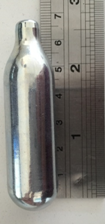
\includegraphics[scale=1]{figures/GasDetectionAgge/SiphonCylinder}
  \caption{A small gas cylinder from a Siphon. Instead gas, it would contain a vacuum}
  \label{fig:Sipon}
\end{figure}

A cylinder of this size has a volume of approximately 13 $cm^3$. This should be enough to let the gasses expand, since most of the liquid water on Europa is expected to be $H_2$O\footnote{\url{http://www.nasa.gov/topics/solarsystem/features/europa20130305.html}, 2016-05-07}, and therefore only a fraction of this is liquid gas. At the top of the cylinder, where it tapers in, the gas is released when punctured. This could be mechanized by a spring, loading the cylinder with nylon string and then burn the nylon string with a small electrode (copper wire) releasing the cylinder into a firing pin, with a small hole in to the test chamber slowly letting the liquid gasses expand.

The liquid under test is contained in the expansion/test chamber, where the vacuum cylinder is connected through the hollow firing pin. The chamber size compared to the vacuum cylinder is the most important ratio, since it determines how low the pressure in the test chamber becomes. The major fact is, as mention, how much liquid "gas" is contained in the water, in the theory section solubility was discussed, but here it was for a gaseousness substance mixed with water and not a liquid gas, further more the pressure is now much higher and Henry's law also needs to be taking into consideration. This part needs further investigation, but for now a good estimate of how much gas that would be in a water sample is 1 \%, this means that 99 \% of the sample is uncompressible. A chamber with a volume of 5 $cm^3$ would contain 0.05 $cm^3$ of liquid gas at 100 bar. To bring this down to 1 bar the volume needs to expand to 5 cm3, more than enough for a vacuum cylinder with a volume of 13 $cm^3$. This gives a satisfying pressure margin of more than 100 \%. Meaning that even with a pressure below the ice of 200 bar the chamber would still be able to reduce the pressure to less than 1 bar. Or if the liquid gas contained in the water is 2 \% of the total volume.

The test chamber needs to be filled and emptied after every use, with inlet and outlet ports in both ends of the chamber. Connected to the inlet and outlet will be a separate solenoid valve, and the pumping system from the other instruments will be utilized to circulate a water sample into the test chamber. The valve system will work by opening the inlet solenoid letting the water fill the chamber, then the valve closes, and the vacuum cylinder is released from its spring mechanism, slowly increasing the volume while the pressure is monitored. The chamber is now at around 1 bar pressure and the outlet valves opens equalizing the pressure, the inlet valve then opens and the chamber is flushed clean. It is very important to thoroughly flush the chamber to avoid any contaminants from previous samples, therefore it is suggested to let the inlet and outlet valve stay open and continually circulate the water surrounding the penetrator, through the chamber. This is of cause only if the sample is taken from the same place all the time, if the penetrator is able to pick up samples from other places then its surroundings a more complex flushing system needs to be implemented.

Lastly the puncture of the cylinder needs to be addressed, as already mention a spring loaded firing pin mechanism, would be the simplest way of implementing the vacuum puncture. This way no motors or valves would be needed, and therefore less points of failure. One of the main problems with this design is to close off the cylinder after the expansion has happened, to avoid that the test chamber volume increase. A way of avoiding this would be the use a two stage spring system, the first stage is fired and punctures the cylinder, when the expansion is done, the next spring fires and blocks the hole with the end of the firing pin.

\begin{figure}[htb]
  \centering
  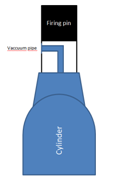
\includegraphics[scale=1]{figures/GasDetectionAgge/Firingpin}
  \caption{The black box is the firing pin where the first part contains the hollow part, which lets the expansion happen, and the solid black is the part that blocks the cylinder after use}
  \label{fig:FiringPin}
\end{figure}

In \ref{fig:FiringPin} an example of such a firing pin is sketched, the box with the black boarder is the firing pin, where the bottom part contains the hollow part, and the top part contains the seal of the cylinder after use. The first stage spring releases and punctures the cylinder, by sending the firing pin down to where the vacuum pipe exits, when the pressure is dropped the next spring releases sealing the cylinder.

The above 4 subsections explains the main parts of the VEGA-instrument, how it works and functions. From this, a hand drawing was made to show how it could look, and to get an idea of the overall dimensions and weight estimate. This first design was made to contain 6 cylinders in a rack structure:

\begin{figure}[htb]
  \centering
  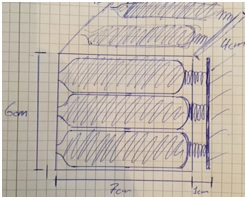
\includegraphics[scale=1]{figures/GasDetectionAgge/CylinderRack}
  \caption{A rack of 6 cylinders, with the spring in the back. Approximate dimensions are 6x8x4cm}
  \label{fig:RackOfSix}
\end{figure}

On \ref{fig:RackOfSix} a sketch of the structure for the cylinders can be seen, in the back the spring system is contained. This rack then connects to the chamber:

\begin{figure}[htb]
  \centering
  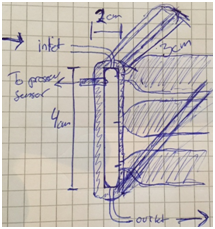
\includegraphics[scale=1]{figures/GasDetectionAgge/ChamberAndRack.png}
  \caption{Cross-section of the chamber and part of the vacuum cylinders, this chamber is 6 $cm^3$ and therefore a little bit too big}
  \label{fig:CrossSectionProto}
\end{figure}

In \ref{fig:CrossSectionProto} a cross section of the chamber is sketched, with part of the cylinder rack. As describe the liquid under test enter through the top inlet and exits at the bottom outlet (the valves are left out). Into the test chamber a pressure sensor is mounted to monitor the expansion. The firing pin is carved into the wall of the chamber and is not visible in the drawing, but when the cylinder is used, the spring will push the cylinder all the way into the wall of the chamber sealing it with the top of the firing pin.

\subsubsection{Principle prototype}

From the drawings and sketches a small prototype was made, which give an idea of how it would look if build. The prototype serves no practical function, and the firing pin or spring system is not build, this is just a chamber with in- and outlet and one cylinder attached.

\begin{figure}[htb]
  \centering
  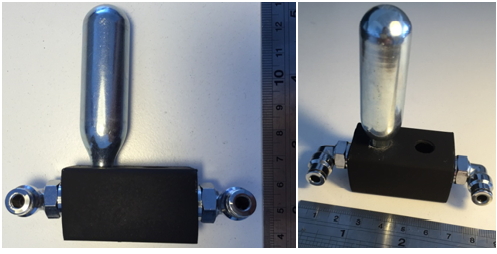
\includegraphics[scale=1]{figures/GasDetectionAgge/Prototype}
  \caption{A non working prototype of the VEGA-instrument. Here with only one cylinder added}
  \label{fig:NonProto}
\end{figure}

If the cylinders are mounted as showed in \ref{fig:NonProto} on the prototype it would be able to contain 7, since one port is used for the pressure sensor. It would be rater bulky due to the mounting of the cylinder on each side; therefore the rack system is more favorable. Overall it gives a good insight in the mechanical construction of the VEGA-instrument.

The last part not discussed is the pressure sensor, here it is possible to use an off the shelve part. Pressure sensors are today already used in harsh environments, and therefore only small modifications might be needed. A good example of a pressure sensor which is small compact and durable is the Festo SPTW-P100R-G14-VD-M12, which is a 0 to 100 bar sensor with a simple threaded connection, which simply screws into the chamber. It might be favorable with a sensor that has a range of 200 bar, but that is easily replaced if deemed necessary. A temperature sensor should also be mounted in the chamber to measure any temperature changes to make sure to get the optimal result.

With the VEGA-instrument not all the gasses specified earlier can be detected, one of the important ones is methane, but this is still a gas at the pressure between 100 and 200 bar, and can therefore not be detected with this expansion method. A way of detecting the methane would be to use a semiconductor sensor as mention in the theory section. This contains no moving parts, and is very simple to use and could be mounted inside the chamber, detecting methane when the chamber is flushed.

\subsubsection{Final physical specification}

When flying a space mission, mass, power consumption and volume of the instrument are very critical, they could be the difference flying the instrument or leaving it.

For the VEGA the configuration of it, inflects on the mass and volume, for this example the instrument carries 6 cylinders, and can therefore be reused 6 times. Dependent on the configuration of the cylinders and the camber the overall volume equates to approximately 200 $cm^3$ without the plumbing and wiring. The mass (build out of titanium) is 180 g for the cylinders, 150 g for the chamber, 120 g for sensor, 200 g for auxiliary. In all 650 g is needed for the whole instrument.

The power consumption for the instrument depends on what stage of use it is in. It does not require any power when not used. When in use the parts that use most power will be the solenoid valve for filling and emptying the chamber, which might draw a few watts when used. The gas sensor also uses a watt or less of power. In all peak consumption is assumed to be 5W, 1W when measuring, and no power use when standby.

There will also be some data processing and data transmission, but this is budgeted by the communication team. The instrument is not heavy on data, a measurement would contain between 5 and 10 Kbytes of data.

\subsection{Conclusion and further work on VEGA-instrument}

Through the design of the VEGA-instrument many different aspects has been covered, to make a comprehensive analysis of how such instrument should be designed for the harsh environment at Europa's ocean. Since this is only a theoretical instrument it is not sure that it will work at the conditions on Europa, therefore more work and test needs to be done. From the sections presented in this report, a prototype needs to be build and tests can begin, to see if it is possible to detect the gasses specified, and if other gasses also can be detected. Also an important aspect of testing is to see how large or small concentrations of a gas it is able to detect, this is dependent on the resolution of the pressure sensor and how much the gas expands when it is boiled of. The result will end up with a redesign of the instrument to accommodate the changes found under test.

Overall the instrument is a reinvention of a gas detector for high pressures, where conventional sensors are not able to work. The solution is simple and rethinks the way of sensing gas; the sensor is not perfect and is limited to a specific number of uses, due to the vacuum cylinders but this is a trade-off between complexity and simplicity. The same goes for the number of gasses it is able to detect, not all gasses can be detected but at the same time it will be able to detect more than compounds specified in this report. If the compound is liquid and mixed with the water, it could detect compounds not expected to be found and therefore the VEGA-instrument can extent it measurement range.


\section{XRF}

\section{Lab-in-a-Chip Systems}


\section{pH \& salinity}

\section{Camera}

\section{Microscope}
